\documentclass[a4paper]{article} 
\addtolength{\hoffset}{-2.25cm}
\addtolength{\textwidth}{4.5cm}
\addtolength{\voffset}{-3.25cm}
\addtolength{\textheight}{5cm}
\setlength{\parskip}{0pt}
\setlength{\parindent}{0in}

\usepackage{charter}
\usepackage[utf8]{inputenc}
\usepackage{microtype}
\usepackage[english]{babel}
\usepackage{amsthm, amsmath, amssymb}
\usepackage{float}
\usepackage[final, colorlinks = true, 
            linkcolor = black, 
            citecolor = black]{hyperref}
\usepackage{graphicx, multicol}
\usepackage{xcolor}
\usepackage{marvosym, wasysym}
\usepackage{rotating}
\usepackage{censor}
\usepackage{listings, style/lstlisting}
\usepackage{pseudocode}
\usepackage{style/avm} 
\usepackage{booktabs}
\usepackage[backend=biber,style=numeric,
            sorting=nyt]{biblatex}
\addbibresource{references.bib}
\usepackage{csquotes}
\usepackage{multirow}
\usepackage[yyyymmdd]{datetime}
\renewcommand{\dateseparator}{-}

\usepackage{fancyhdr} 
\pagestyle{fancy} 
\fancyhead{}\renewcommand{\headrulewidth}{0pt}
\fancyfoot[L]{Udacity Machine Learning Engineer Nanodegree}
\fancyfoot[C]{}
\fancyfoot[R]{\thepage}

\newcommand{\note}[1]{\marginpar{\scriptsize \textcolor{red}{#1}}}

\begin{document}
\title{template_assignment (ECL)}
\fancyhead[C]{}
\hrule \medskip 
\begin{minipage}{0.295\textwidth}
\raggedright
Udacity\\ 
\footnotesize 
\hfill\\
Luiz Alberto Ferreira Gomes
\end{minipage}
\begin{minipage}{0.4\textwidth} 
\centering 
\large 
Project Report\\ 
\normalsize 
Machine Learning Engineer Nanodegree\\ 
\end{minipage}
\begin{minipage}{0.295\textwidth} 
\raggedleft
\today\\ 
\footnotesize 
\hfill\\
gomes.luiz@gmail.com 
\end{minipage}
\medskip\hrule 
\bigskip

%\begin{multicols}{2}
%[
\section{Project Overview}
Bug Report Tracking Systems(BTS), such as Bugzilla or Jira, have played a major role in the maintenance process in many software development settings, both in Closed Source Software (CSS) and in Open Source Software (OSS). This fact is especially true in OSS projects -- characterized by many users and developers with different levels of expertise spread out the world -- who might create or be responsible for dealing with several bug reports. A user interacts with a BTS often through a simple mechanism called bug report form\cite{Tian:2012}. This kind of form enables users to request changes, to report bugs, or to ask for support in a software product. Initially, he or she should inform a short description, a long description, a type (e.g., bug, new feature, improvement, and task), and an associated severity level (e.g., blocker, critical, major, minor, and trivial). Subsequently, a development team member will review this request and, in case it is not refused for some reason (e.g., bug report duplication), he or she will complete the information in bug report form, indicating, for example, its severity and assigning the person responsible for the bug report. \cite{Cavalcanti:2014}. In this context, my project built a machine learning web application for bug severity prediction based on the bug description filled by users when they open a bug.

\subsection{Problem Statement}
The severity level information is recognized as a critical variable in the equation to estimate a prioritization of bugs. It defines how soon the bug report needs to be addressed. However, the severity level assignment remains mostly a manual process that relies only on the experience and expertise of the person who has opened the bug report~\cite{Yang:2017}. As a consequence, it is a process with a high degree of subjectivity, and it may be quite error-prone. The number of bug reports in large and medium software OSS projects is frequently very large. Severity level shifts throughout the bug report lifecycle may harm the planning of maintenance activities. For example, the maintenance team could be assigned to address less significant bug reports before the most important ones.

\bigskip

\section{Solution Statement}
The general purpose of my project is to develop an intelligent ML-based web assistant to help developers and maintenance team to predict the severity level of a bug (blocker, critical, major, minor, or trivial). To meet the goal, the tasks that were executed are the following:
\begin{enumerate}
    \item Collect bug reports data from a Bugzilla BTS;
    \item Pre-process the description text using text mining techniques (e.g. tokenization).
    \item Train and test a machine learning classifier to predict bug severity level based on bug report description;
    \item Build and deploy a web application to extract a bug report description from a Bugzilla BTS and predict the bug severity level.
\end{enumerate}
%]
\subsection{Datasets and Inputs}
I've used a dataset with 2395 bug reports, collected from Mozilla project and available in the project GitHub repository\footnote{\url{https://github.com/gomesluiz/bug-severity-predictor/blob/main/data/raw/mozilla_bug_report_data.csv}}, to train and test the predicting model. The Mozilla project encompasses several open-source projects, such as Firefox, Thunderbird, and Bugzilla. Furthermore, it is well-established, has a considerable number of registered bug reports, uses standard repositories, and were being studied in academic research~\cite{Lamkanfi:2010, Lamkanfi:2011, Tian:2012}. Table~\ref{tab:features_descriptions} describes the features of the dataset that will used for bug report severity prediction. Each feature in this table has a description, a category.

\begin{table}[ht!]
    \centering
    \begin{tabular}{@{}p{.20\textwidth}p{.30\textwidth}p{.15\textwidth}p{.10\textwidth}@{}}
    \toprule
    {\bf Feature} & {\bf Description} & {\bf Category} & {\bf Target Label}\\
    \midrule
    Bug id                       & Bug report identifier.  & Quantitative Discrete & No\\
    \midrule
    Description                  & Textual content appearing in the description field of the bug report.                                                                               & Unstructured Text & No\\
    \midrule
    Severity                     & Indicates how severe the problem is – from blocker (``application unusable”) to trivial (``minor cosmetic issue”).                                & Qualitative Ordinal & Yes\\
    \bottomrule 
    \end{tabular}
    \caption{The features and its descriptions of dataset used for bug severity prediction. The target label of prediction model is the {\bf Severity} feature }\\
    \label{tab:features_descriptions}
\end{table}


\bigskip
Figure~\ref{fig:severity_class_distribution} shows the label distribution in the Mozilla dataset, which will be used to train and test the prediction model. It will be split into a training set (75\% out of 2395) and into a testing set (25\% out of 2395). As one can observe, the label distribution in the dataset is unbalanced. Therefore, to maintain the proportion of labels in training and testing sets, I will use the stratify splitting and class weighting\cite{procrastinator:2021} to mitigate the unbalancing impact.

\begin{figure}[ht!]
    \centering
    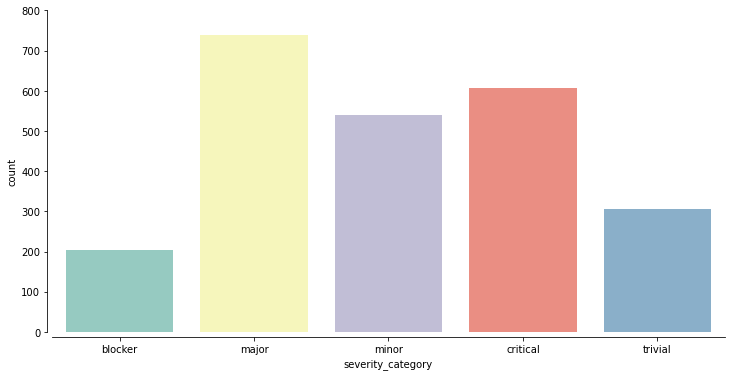
\includegraphics[width=0.8\textwidth]{figures/severity-labels-distribution.png}
    \caption{Target label distribution on the Mozilla bug reports dataset.}
    \label{fig:severity_class_distribution}
\end{figure}

\subsection{Evaluation Metrics}
The specific metrics I'll use for assessing prediction performance for evaluating the accuracy of classification algorithms will be precision, recall, and F-measure, described as follows\cite{Kuhn:2013}:

\begin{itemize}
\item \textbf{Recall}. The recall is the number of True Positives (TP) divided by the number of True Positives (TP) and of False Negatives (FN), where the TP and FN values are derived from the confusion matrix. A low recall indicates many false negatives.

\item \textbf{Precision}. Precision is the number of True Positives (TP) divided by the number of True Positives and False Positives (FP). A low precision can also indicate many false positives.

\item \textbf{F-measure}. F-measure conveys the balance between precision and recall and can be calculated as their harmonic mean. 
\end{itemize}

The metrics above especially useful when the target classes are unbalanced, which often happens in many settings, such as bug severity prediction. Also, these metrics enable the comparison between my prediction model and benchmark models.

\subsection{Benchmark model}

The benchmark model that will be used in my project will be based on the literature. Table \ref{tab:performance_of_algorithms}  provides a quantitative view of the performance obtained in the experimental setting, showing the algorithms which presented the best performances in some papers. 

\begin{table}[htp]
        \scriptsize
        \centering
        
        \begin{tabular}{@{}p{.10\textwidth}p{.10\textwidth}p{.20\textwidth}p{.10\textwidth}ccccc@{}}
        \toprule
        \multirow{2}{*}{\thead{Ref.}} & \multirow{2}{*}{\thead{Projects}} & \multirow{2}{*}{\thead{Algorithms}} & \multirow{2}{*}{\thead{Hyper\\parameters}} & \multirow{2}{*}{\thead{Classes}} & \multicolumn{1}{c}{\thead{}} & \thead{Metrics}         & \thead{}          & \multirow{2}{*}{\thead{Terms}} \\ \cmidrule(lr){6-8}
                                            &                                   &                             &  & & \thead{AUC}                        & \thead{Accuracy} & \thead{F-Measure} &                                           \\ \cmidrule(r){1-5} \cmidrule(r){6-8} \cmidrule(l){9-9} 
    
        \cite{Yang:2012}                    &  Mozilla                          &  Multinomial Näive Bayes                        &  & 2 & 0.849                               &                   &                    & 100                                          \\ 
        \cmidrule{1-9}    
        \cite{Yang:2014b}                   &  Mozilla                          &  KNN                        & K = 1 & 7 &                                     &  0.750           &                    & 40                                          \\ 
        \cmidrule{1-9}
        \cite{Valdivia:2014}                &  Mozilla                          &  Random Forest              &  & 2 &                                     &  0.823            &  0.432             &                                           \\ 
        \cmidrule{1-9}
        \cite{Meera:2014}                   &  Mozilla                          &  Näive Bayes                         &  & 6 &                                     &  0.916            &                    &                                           \\ 
        \cmidrule{1-9}
        \cite{Roy:2014}                     &  Mozilla                          &  Näive Bayes                         &  & 2 & 0.924                               &  0.880                 &  0.797                & 750                                          \\ 
        \cmidrule{1-9}
        \cite{Xia:2015}                     &  Mozilla                          &  Bagging Ensemble           &  & 2 &                                     &                   &  0.482             &                                           \\ 
        \cmidrule{1-9}
        \cite{Pushpalathas:2016}            &  Mozilla                          &  Bagging Ensemble           &  & 4 &                                     &  0.812            &                    &                                           \\ 
        \cmidrule{1-9}
        \cite{Otoom:2016}                   &  Mozilla                  &  Random Forest              &  & 2 &                                     &  0.764            &                    & 59                                          \\ 
        \cmidrule{1-9}
        \cite{Jin:2016a}                    &  Mozilla                               &  Multinomial Näive Bayes                        &  & 2 &                                     &                   &    0.820                &  79,000                                         \\ 
        \cmidrule{1-9}
        \cite{Jin:2016b}                    &  Mozilla                          &  Multinomial Näive Bayes                       &  & 2 &                                     &                   &  0.820             &                                           \\ 
        \cmidrule{1-9}
        \cite{Jin:2016c}                    &  Mozilla                          &  Multinomial Näive Bayes                        &  & 2 &                                     &     &  0.790             &                                           \\ 
        \bottomrule
        \end{tabular}
        \caption{The best ML algorithms performance of papers in the literature.}
        \label{tab:performance_of_algorithms}
    \end{table}

\noindent\fbox{%
    \parbox{\textwidth}{%
        I've built the severity prediction model using only {\bf 1000} bug reports (750 for training and 250 for testing) because of the \underline{computer resource limitation}. Even so, This model, considering {\bf five classes}, yielded an F-measure from {\bf 7\% (blocker)} to {\bf 47\% (critical)}, which are promising and are compatible with the results shown in Table \ref{tab:performance_of_algorithms}.
    }%
}

\section{Project Design}
Figure~\ref{fig:application-architecture} shows the high-level architecture of the bug severity predictor application. The architecture will consist of two modules: front-end and back-end modules. The front-end module will run in a web browser, and it will be in charge of receiving and displaying data from or to the user. The back-end module will run in a server and be responsible for cleaning, breaking into tokens, and weighting each term of the bug description text extracted from a BTS system. Moreover, the back-end module will predict the bug severity level, as requested of the front-end, based on the bug description and the predicting model previously saved. The front-end module will communicate with the back-end throughout the REST protocol. 
\begin{figure}[h!]
    \centering
    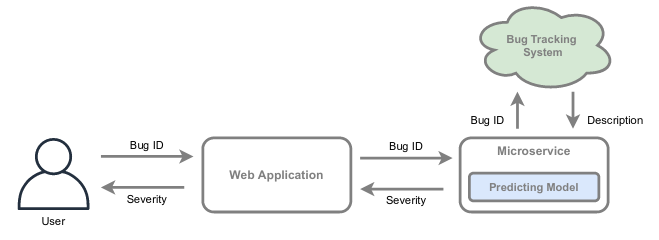
\includegraphics[width=0.8\textwidth]{figures/architecture-overview.png}
    \caption{High-level architectural design.}
    \label{fig:application-architecture}
\end{figure}

The predicting model will be train and test using features extracted using the Pre-training of Deep Bidirectional Transformers for Language Understanding (BERT)\cite{devlin:2019}.

\bigskip
Figure~\ref{fig:machile-learning-workflow} shows the main activities of the project to implement the proposed architecture above, which are described as the following:

\begin{enumerate}
    \item {\bf Clean, tokenize and weight the description feature:} This activity cleaned and tokenized the description feature of the Mozilla dataset. Next, it weighted the tokens of each cleaned description. To do that, I used the NLTK Python library and BERT deep neural network architecture. 
    
    \item {\bf Split the dataset:} This activity split the processed dataset in training~(75\%), and testing sets~(25\%). To do that, I used the Scikit-learn Python library. 
    
    \item {\bf Train and tune the model:} This activity trained and tuned the predicting model. To train, I used the XGBoost algorithm from the Scikit-learn library, and, to tune, I used the Distributed Asynchronous Hyperparameter Optimization (Hyperopt).
    
    \item {\bf Calculate and evaluate training metrics:} This activity calculated and evaluated training metrics. To calculate metrics I've used the methods from the Scikit-learn library.
    
    \item {\bf Test and evaluate the model:} This activity tested and evaluated the predicting model. To test, I've used methods from the Scikit-learn library, and, to evaluate, I've used the methods from the Scikit-learn library.
    
    \item {\bf Calculate and evaluate testing metrics:} This activity calculated and evaluated testing metrics. To calculate metrics I'll the methods from the Scikit-learn library and, to evaluate, I've used the methods from the Scikit-learn library.
    
    \item {\bf Deploy in production:} This activity deployed a model in a web application in the cloud. To develop the application, I've used the Flask Python library for the back-end, and HTML, Javascript, and CSS for the front-end.
    
\end{enumerate}

%\begin{table}[h!]
%    \centering
%    \begin{tabular}{@{}ll@{}}
%    \toprule
%    {\bf Module/Funcionality} & {\bf Technology/Library}                       %  \\ \midrule
 %   Front-end/User Interaction           & HTML, CSS, Javascript/Bootstrap    %       \\
 %   Back-end/Microservices            & Python/Flask                          %    \\
 %   Back-end/Predicting and Modeling & Python/Scikit-learn, Tensorflow, and Bert \\
 %   Back-end/Text mining         & Python/NLTK                               \\
 %   Back-end/Web scrapping       & Python/Scrapy                             \\ \bottomrule
  %  \end{tabular}
  %  \caption{Summary of technologies and libraries that will be used in the current project.}
 %   \label{tab:techology_summary}
%\end{table}

\begin{figure}[h!]
    \centering
    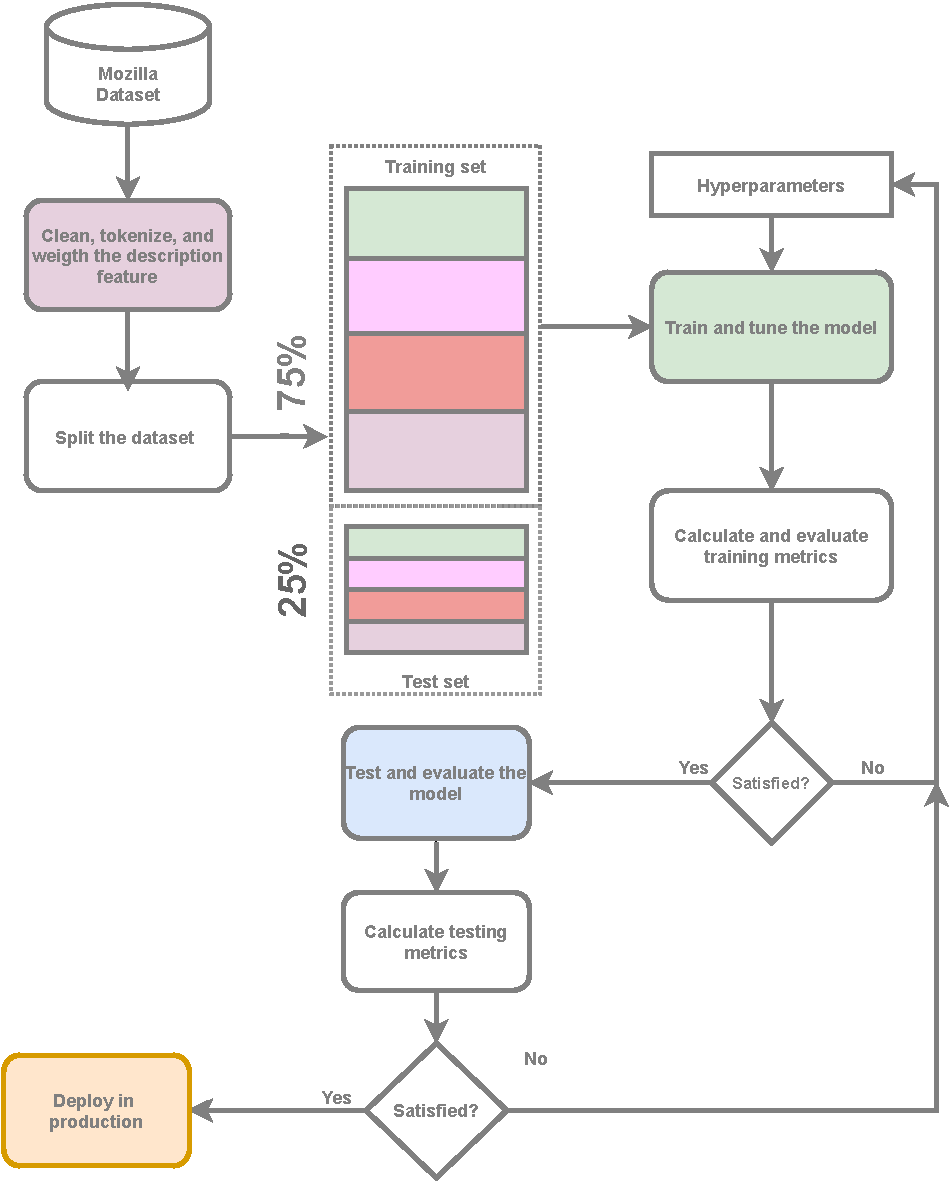
\includegraphics[width=0.5\textheight]{figures/machine-learning-worflow.pdf}
    \caption{Machine learning workflow of the projetc.}
    \label{fig:machile-learning-workflow}
\end{figure}

\subsection{Web Application}
Figure~\ref{fig:succes-prediction} shows the application screen when a successful bug severity prediction was executed.

\begin{figure}[h!]
    \centering
    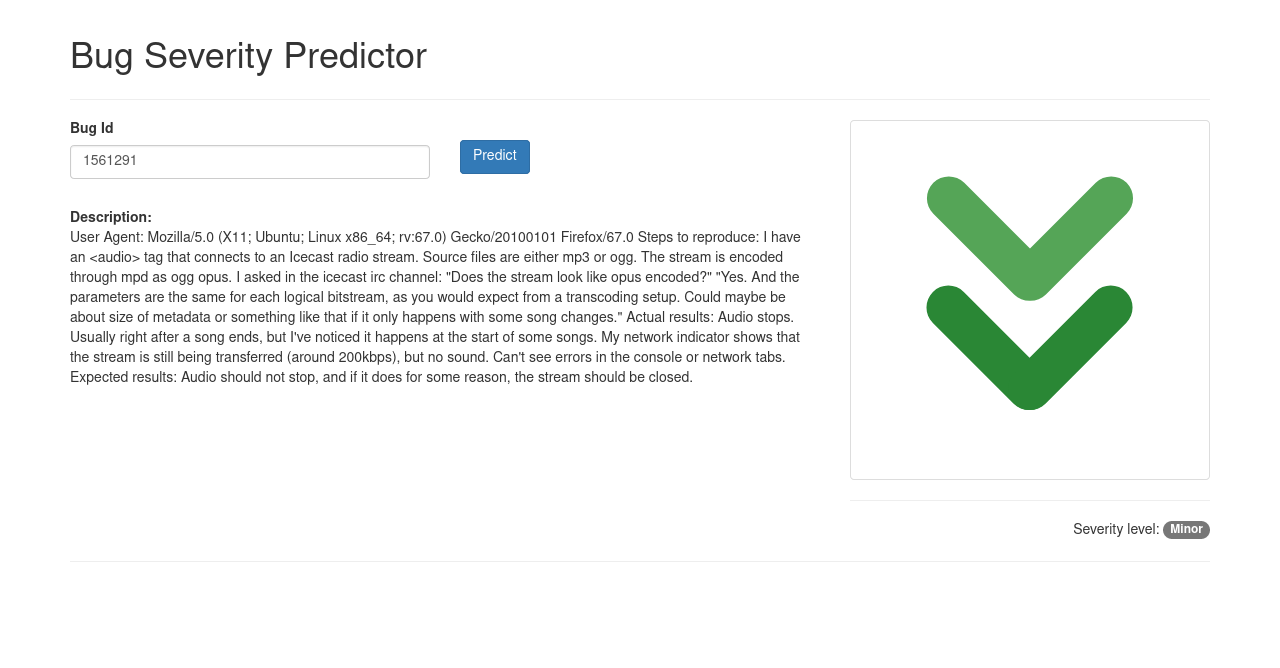
\includegraphics[width=0.8\textwidth]{figures/sucess-prediction.png}
    \caption{A successful bug severity prediction.}
    \label{fig:succes-prediction}
\end{figure}

Figure~\ref{fig:failed-prediction} shows the application screen when a failed bug severity prediction was executed because the bug does not exist in Mozilla BTS.

\begin{figure}[h!]
    \centering
    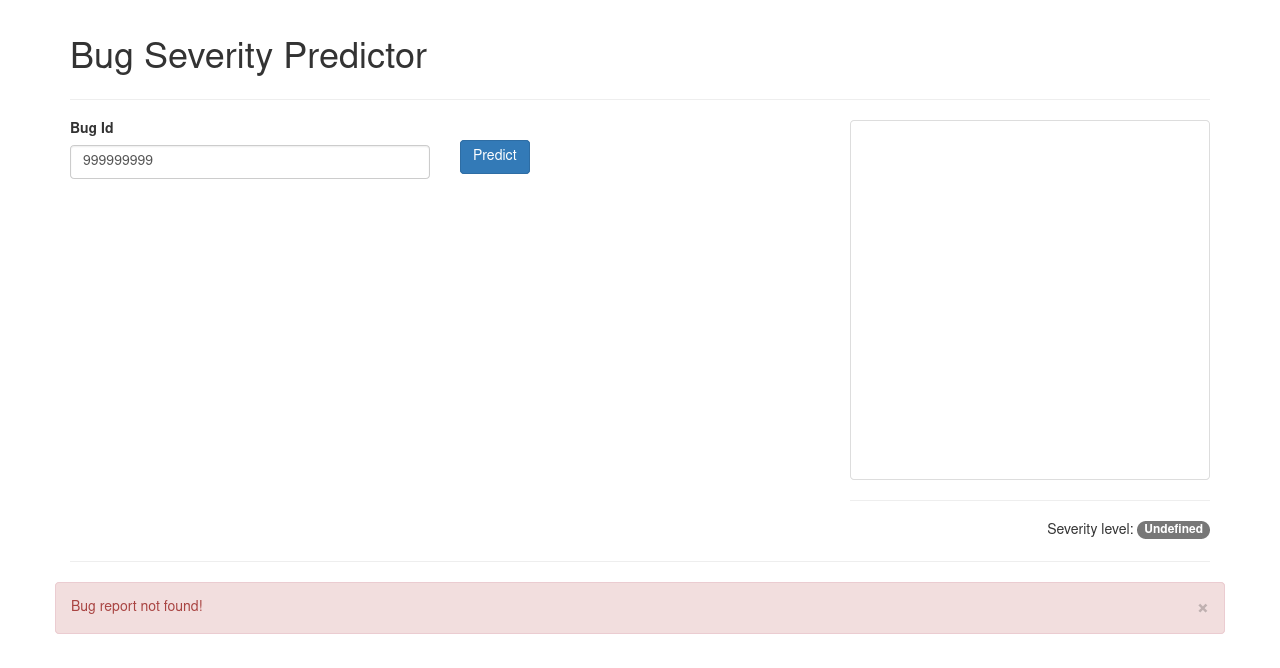
\includegraphics[width=0.8\textwidth]{figures/failed-prediction.png}
    \caption{Caption}
    \label{fig:failed-prediction}
\end{figure}

\section{Conclusion}
In this project, I have built a web application to predict the bug severity level for Mozilla bug reports. The predicting model of this application was based on the XGBoost ML algorithm on an imbalanced data scenario. Furthermore, I've used the BERT, a pre-training deep neural network, to extract feature vectors considering the 128 tokens of each bug report description and the Distributed Asynchronous Hyperparameter Optimization (Hyperopt) to select the best XGBoost hyperparameters.  The evaluation of the application prediction model, considering only 1000 bug reports and five severity levels, has yielded was around from 7\% (blocker) to 47\% (critical), which was a promising result and compatible with literature.
  

\newpage
\bigskip
\printbibliography

%----------------------------------------------------------------------------------------

\end{document}
